Spell checking: aspell -c -t summary.tex -d en

xelatex DevThesis
bibtex DevThesis

\section{Introduction}
\subsection{Parallels research}

This section section just some examples of various types of Latex things that can be used.

\begin{enumerate}
 \item Adding more texts
 \item Adding cross-language parallels
 \item Further development of the website UI
\end{enumerate}

\newpage

\rotatebox{90}{\includegraphics[width=\textheight,height=\textwidth,keepaspectratio]{timeline.pdf}}

\includegraphics[width=\linewidth]{textview1.png}
\captionof{figure}{The website displaying T1600 (辯中邊論) as the main text in text view mode.}
\label{textview1}

\medskip
Figure \ref{textview1}

\footnote{this solution, rather by coincidence, is similar to the solution presented in (\cite{sturgeon2017}), where different shades of red were used to indicate layers of quotations. However, unlike (\cite{sturgeon2017}) in this study the differences in wordings between two passages are not visually highlighted. This is due to the fact that the data also contains examples of less verbatim quo-
tations, where such a mechanical highlighting strategy becomes difficult to apply.}


Two images next to each other:
\begin{figure}[!tbp]
  \centering
  \subfloat[Palace eunuchs in ancient China]{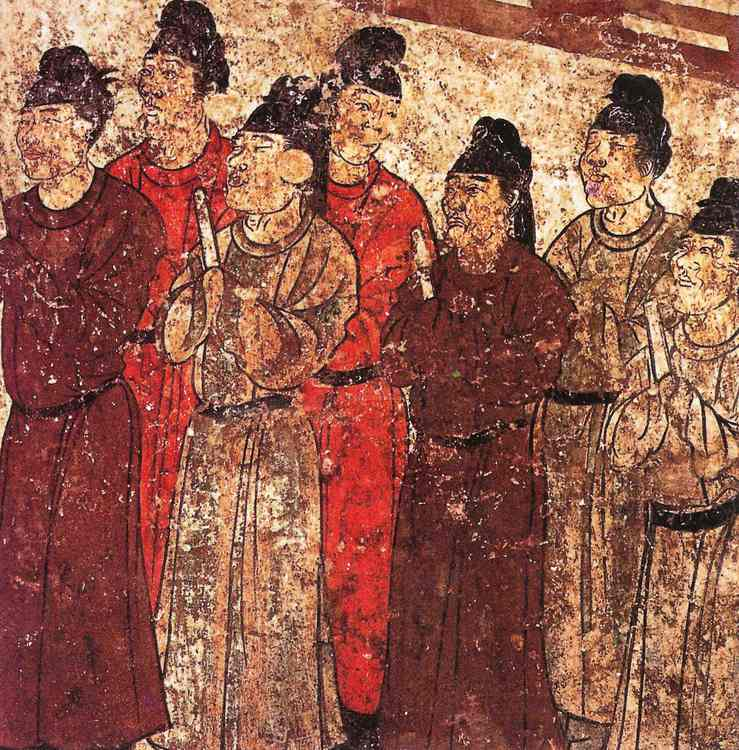
\includegraphics[width=0.4\textwidth]{Eunuchs-in-ancient-China.jpg}}
  \hfill
  \subfloat[Hijra in India]{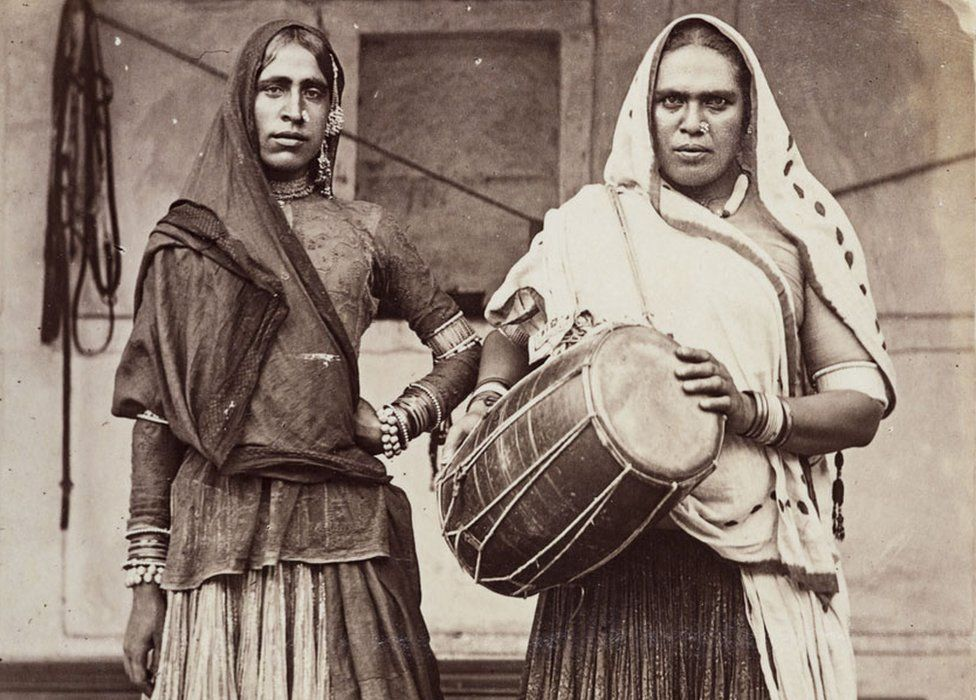
\includegraphics[width=0.4\textwidth]{hijra.jpg}}
\end{figure}



\begin{tabular}{ c c c }
 \textbf{Description} & \textbf{Monthly costs (USD)} & \textbf{Annual costs (USD)} \\ 
 Part-time developer & 3.000 & 36.000 \\  
 \href{https://www.linode.com/pricing}{VPS Linode 4G plan} & 20 & 240 \\
  \href{https://www.linode.com/blockstorage}{500 GB storage} & 50 & 600 \\
  3x Nvidia RTX 2080 TI GPU & - & 3600 \\
  TPU training Google cloud (opt) & - & 1500 \\
 \textbf{Total costs} & & \textbf{41.940}
\end{tabular}


Donald \cite{sturgeon2017} points out in his article {\em `Unsupervised identification of text reuse in early Chinese literature'}: 

\begin{quote}
A further observation emerging from this study is that a key advantage of digital systems over traditional printed forms of research lies in the possibility of allowing scholars to work with all data of a particular kind, rather than a useful and important subset selected by experts. With the sheer volume of parallels spread throughout the early Chinese corpus, even the most diligent of conventional studies risks omitting information that may prove relevant to the particular research questions that someone else may be interested in.
\end{quote}
